\subsection{Data collection \& management}

We have developed a new platform that allows housing of mice in large arenas
(\textgreater 2m diameter), while manipulating and monitoring their behaviour
at high spatiotemporal resolution \citep[Figure~\ref{fig:arena}, ][]{campagnerEtAl24}.
%
We have openly shared software for supporting data acquistion
\citep{aeonacquisition} and management \citep{aeonmecha} in this
arena.
%
Using this platform we have collected several week long datasets both with
single mouse and multiple mice.
%
These datasets capture a rich behavioural repertoire including a foraging
behaviour,  social learning task, defensive and nesting behaviours.


\begin{figure}
    \centering
    \subfloat[]{
        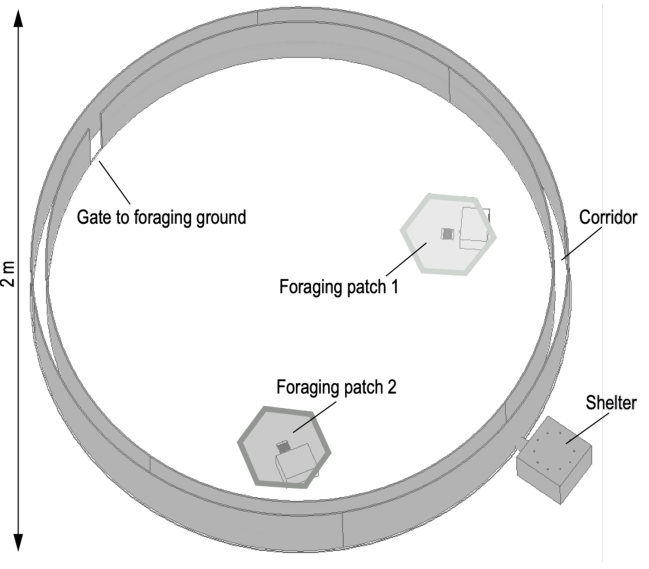
\includegraphics[width=4in]{figures/arena.png}
    }
    \hfill
    \subfloat[]{
        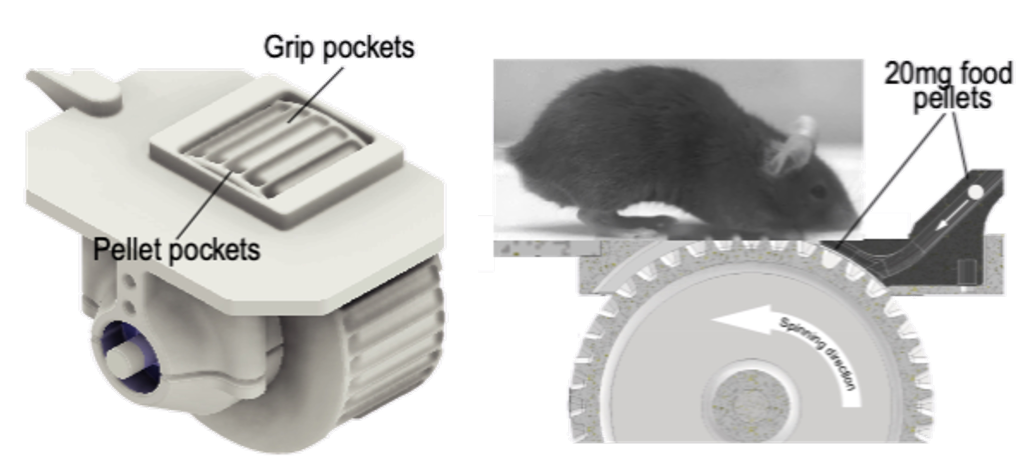
\includegraphics[width=4in]{figures/patch.png}
    }
    \caption{Foraging Arena (a) and Feeder (b).
    %
    The arena is composed of tessellated hexagonal tiles (a), each featuring a
    newly designed underground feeder (b).
    %
    Pellets are dispensed onto a foraging wheel once the mouse has spun it for
    a pre-defined programmable distance threshold using its forepaws (fictive
    digging).
    %
    The arena contains up to six scale-equipped nesting modules that allows
    housing of mice in the arena and weight monitoring.
    %
    Behavioural monitoring is achieved by an array of high-speed cameras (up to
    15), by which mouse location, mouse identity and body parts can be track in
    real time.
    %
    }
\label{fig:arena}
\end{figure}


\subsection{Data sharing}

The large dataset sizes generated by NaLoDuCo experiments, on the order of
hundreads of terabytes,  make it impractical to distribute data to users, and
require to bring users to data. Fortunately, cloud technologies are now mature
to allows this.
%
We will store data in the Distributed Archives for Neuroscience Data
Integration (DANDI), which uses Amazon S3 buckets, and we will provide software
to visualize and analyze data in Amazon EC2 instances, to avoid costly data
transfers.

CatalystNeuro has played a pivotal role in supporting the development and
operations of DANDI.

\subsection{Data visualisation}

Visualisations are essential for scientific discovery. Our visualisation tools
need to display very large datasets at different temporal scales, from
milliseconds to weeks and months, and they need to be web based.
%
We will use multi-resolution visualization techniques, which store data at
various resolutions, and use the approriate resolution for each zoom level.
%
Web-based visualisation will be optimized using web workers
\cite{webWorkers}.

Dr.~Magland has extensive experience buidling web based visualizations (e.g.,
Neurosift \cite{neurosift})

\subsection{Spike sorting}

Spike sorting is specially challenging in NaLoDuCo experimentation since we
want to track individual neurons of freely moving mice for weeks to months.
%
In addition, spike sorting needs to be done online, to allow experiments driven
by real-time machine learning inference, as described below.
%
Furthermore, sorting algorithms need to operate on probes with hundreads of
channels.

Methods have been proposed for tracking neurons for long periods of time (e.g.,
\cite{yuanEtAl24,vanBeestEtAl24}) and for online sorting (e.g.,
\cite{rutishauserEtAl06,santhanamEtAl04}). We will rigorously evaluate these
methods and report the results of these evaluation, so that researchers can
choose the method that best fits their needs.

Prof.~Sahani pioneered the use of Bayesian inference methods for spike sorting
\cite{sahani99}. Dr. Jeremy Magland has significantly advanced the field of
spike sorting, particularly through his development of MountainSort
\cite{mountainSort5} and his contributions to
SpikeInterface\cite{spikeInterface}.

\subsection{Data analysis}

Analyzing NaLoDuCo experimental data is challenging for at least two reasons.
%
First, conventional machine learning methods operate offline (i.e., they load
into memory data previously recorded, process it, and save the analysis
results).
%
These batch methods cannot be used in NaLoDuCo experiments, as the very large
datasets from these experiments cannot be loaded into memory.
%
Intead, NoDoLuCo experiments require \textbf{online methods}, that can process
infinite data steams.

Second, a pervasive assumption in most ML algorithms is stationarity; i.e., the
assumption that the statistics of data do not change over time.
%
But in long-duration and continuous experiments this assumption is most often
violated as, for example, the arousal of subjects changes.
%
Hence, the analysis of data generated by these experiments requires
\textbf{adaptive methods}.

We have identified a few data analysis problems in NaLoDuCo experimentation
(described in the following subsections) to be addressed with machine learning
methods.
%
For each of these problems we will evaluate different ML algorithms, carefully
document the results of the evaluations, and create a benchmark comparing
evaluated models.
%
We want to know, and let others know, which method performs the best for
NaLoDuCo experimentation.

